\subsection{Detector Optimization}
\label{sec:codesign}
%\textbf{\emph{Cristiano}}


Detector optimization is an essential part of the R\&D and design process that involves mechanical design and budget to realize the best performance possible.  
This process is anticipated to continue in the months following the detector proposal towards CD-2 and CD-3. 

Optimizing the design of large scale detectors like ECCE made by multiple sub-detector systems is a complex problem. 
Each sub-detector system is in fact characterized by a multi-dimensional design parameter space (describing, \textit{e.g.}, geometry, mechanics, optics, etc). 
In addition to that, detector simulations are typically computationally intensive, as we need to rely on advanced simulation platforms used in our community like Geant \cite{Agostinelli:2002hh} to simulate the interaction of radiation with matter. 

In the past the typical workflow during the design phase consisted in characterizing each sub-detector individually by taking into account constraints from the whole global detector design.
The optimization was usually carried out manually or with brute-force methods considering only one figure of merit. Eventually all sub-detectors were combined together.
Nowadays state of the art techniques based on AI can provide dedicated strategies for complex combinatorial searches. 
These algorithms are particularly useful to efficiently explore a usually large solution space and to minimize the computational budget needed to converge to these optimal solutions. 

The typical software stack that is utilized in the detector design process involves three main steps:
(i) generation of events, (ii) detector simulations
and (iii) reconstruction and analysis. 
%
A sequential AI-based strategy in general gathers the information associated to the proposed design point, \textit{i.e.} some figures of merit that quantify the goodness of the design, and based on this information suggests which design parameters to query at the next iteration. This scheme is shown in Fig.~\ref{fig:design_AI}. 
%
A first parallelized, automated and self-consistent AI-supported strategy for detector optimization has been demonstrated for the dual-RICH by \cite{cisbani2020ai} leveraging Bayesian optimization (BO) \cite{snoek2012practical}. 
A workflow of this framework is shown in Fig.~\ref{fig:dRICH_BO_scheme}, where more details can be found. 



\begin{figure}[!]
    \centering
    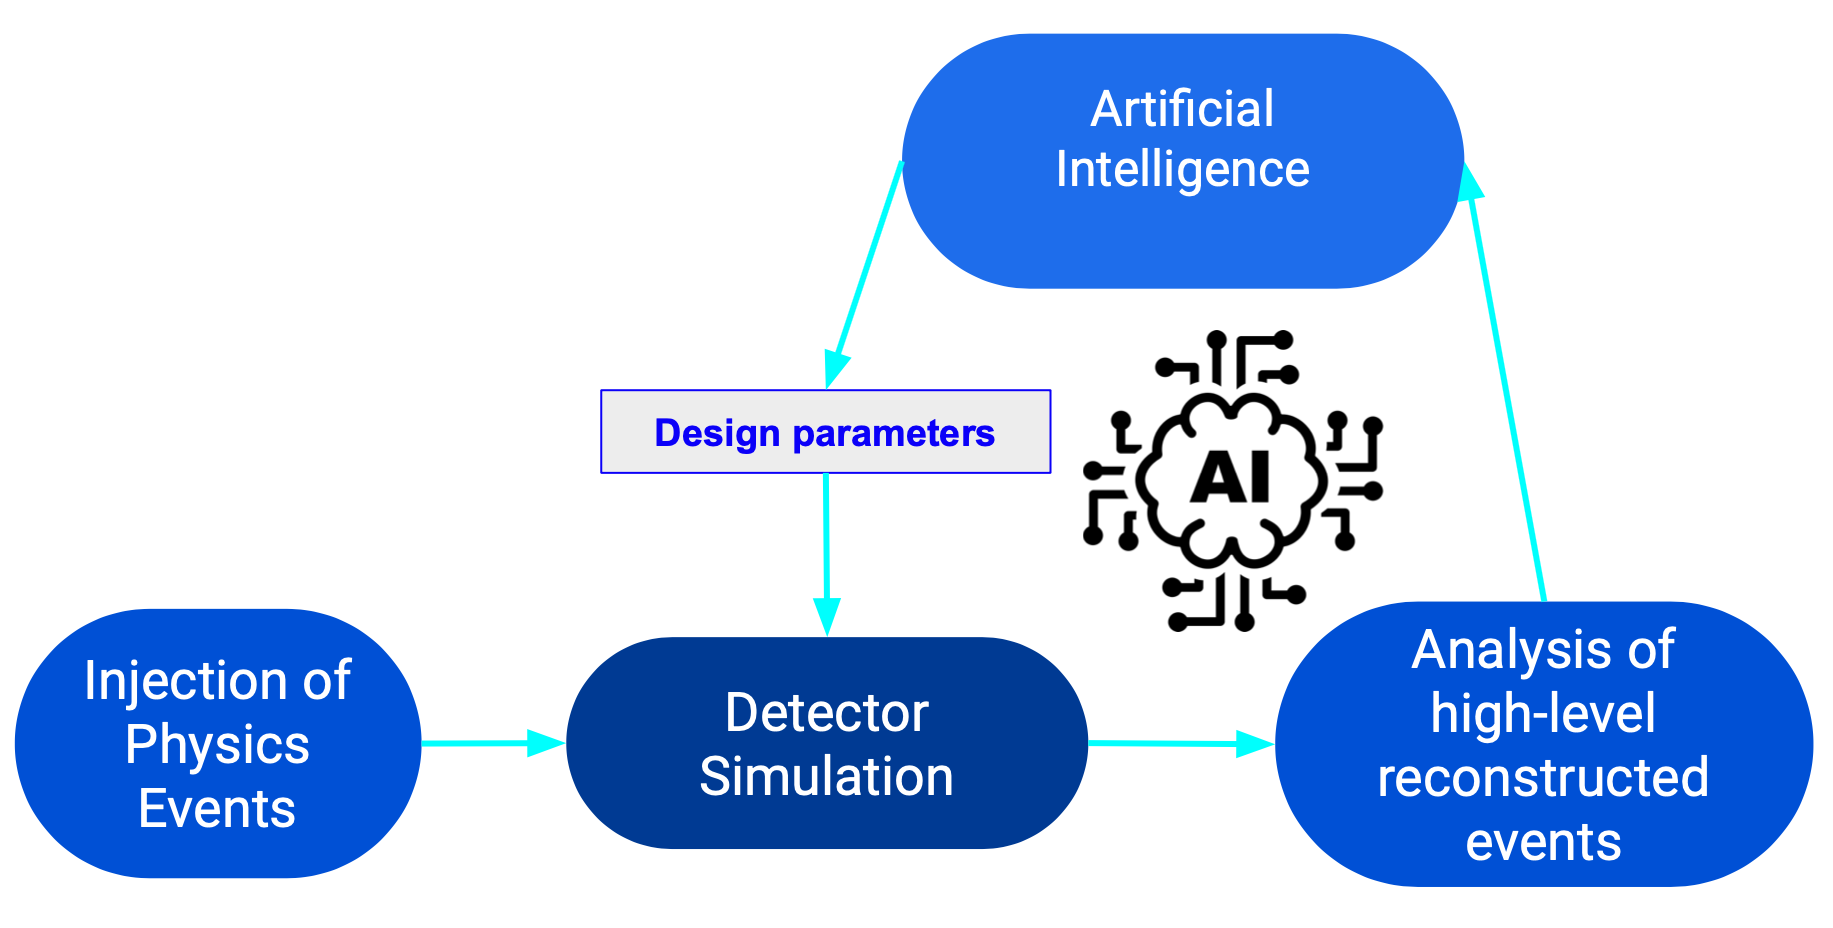
\includegraphics[scale = 0.18]{figs/design_workflow.png}
    %\includegraphics[scale = 0.15]{figs/ECCE_teams.png}
    \caption{%(top) 
    Typical workflow of detector design assisted by AI: physics events are injected in a detector characterized by some given design parameters. Reconstructed events are analyzed and figures of merit are quantified and passed to some AI-based strategy, which in turn suggests the next design point to observe in this sequential approach; notice that AI can also intervene in the simulation and reconstruction steps. %(bottom) AI fosters the interplay between the Detector, Physics and Computing Teams in ECCE: the Physics Team provides physics generators and is responsible for the evaluation of performance after reconstruction; the Detector Team is responsible of the selection of technology, the choice of the updated baseline design, and the proposal of alternative configurations; the Computing Team offers the support in producing the simulation campaign, as well as the optimization pipeline of each new alternative detector configuration.
    }
    \label{fig:design_AI}
\end{figure}

\begin{figure}[!]
    \centering
    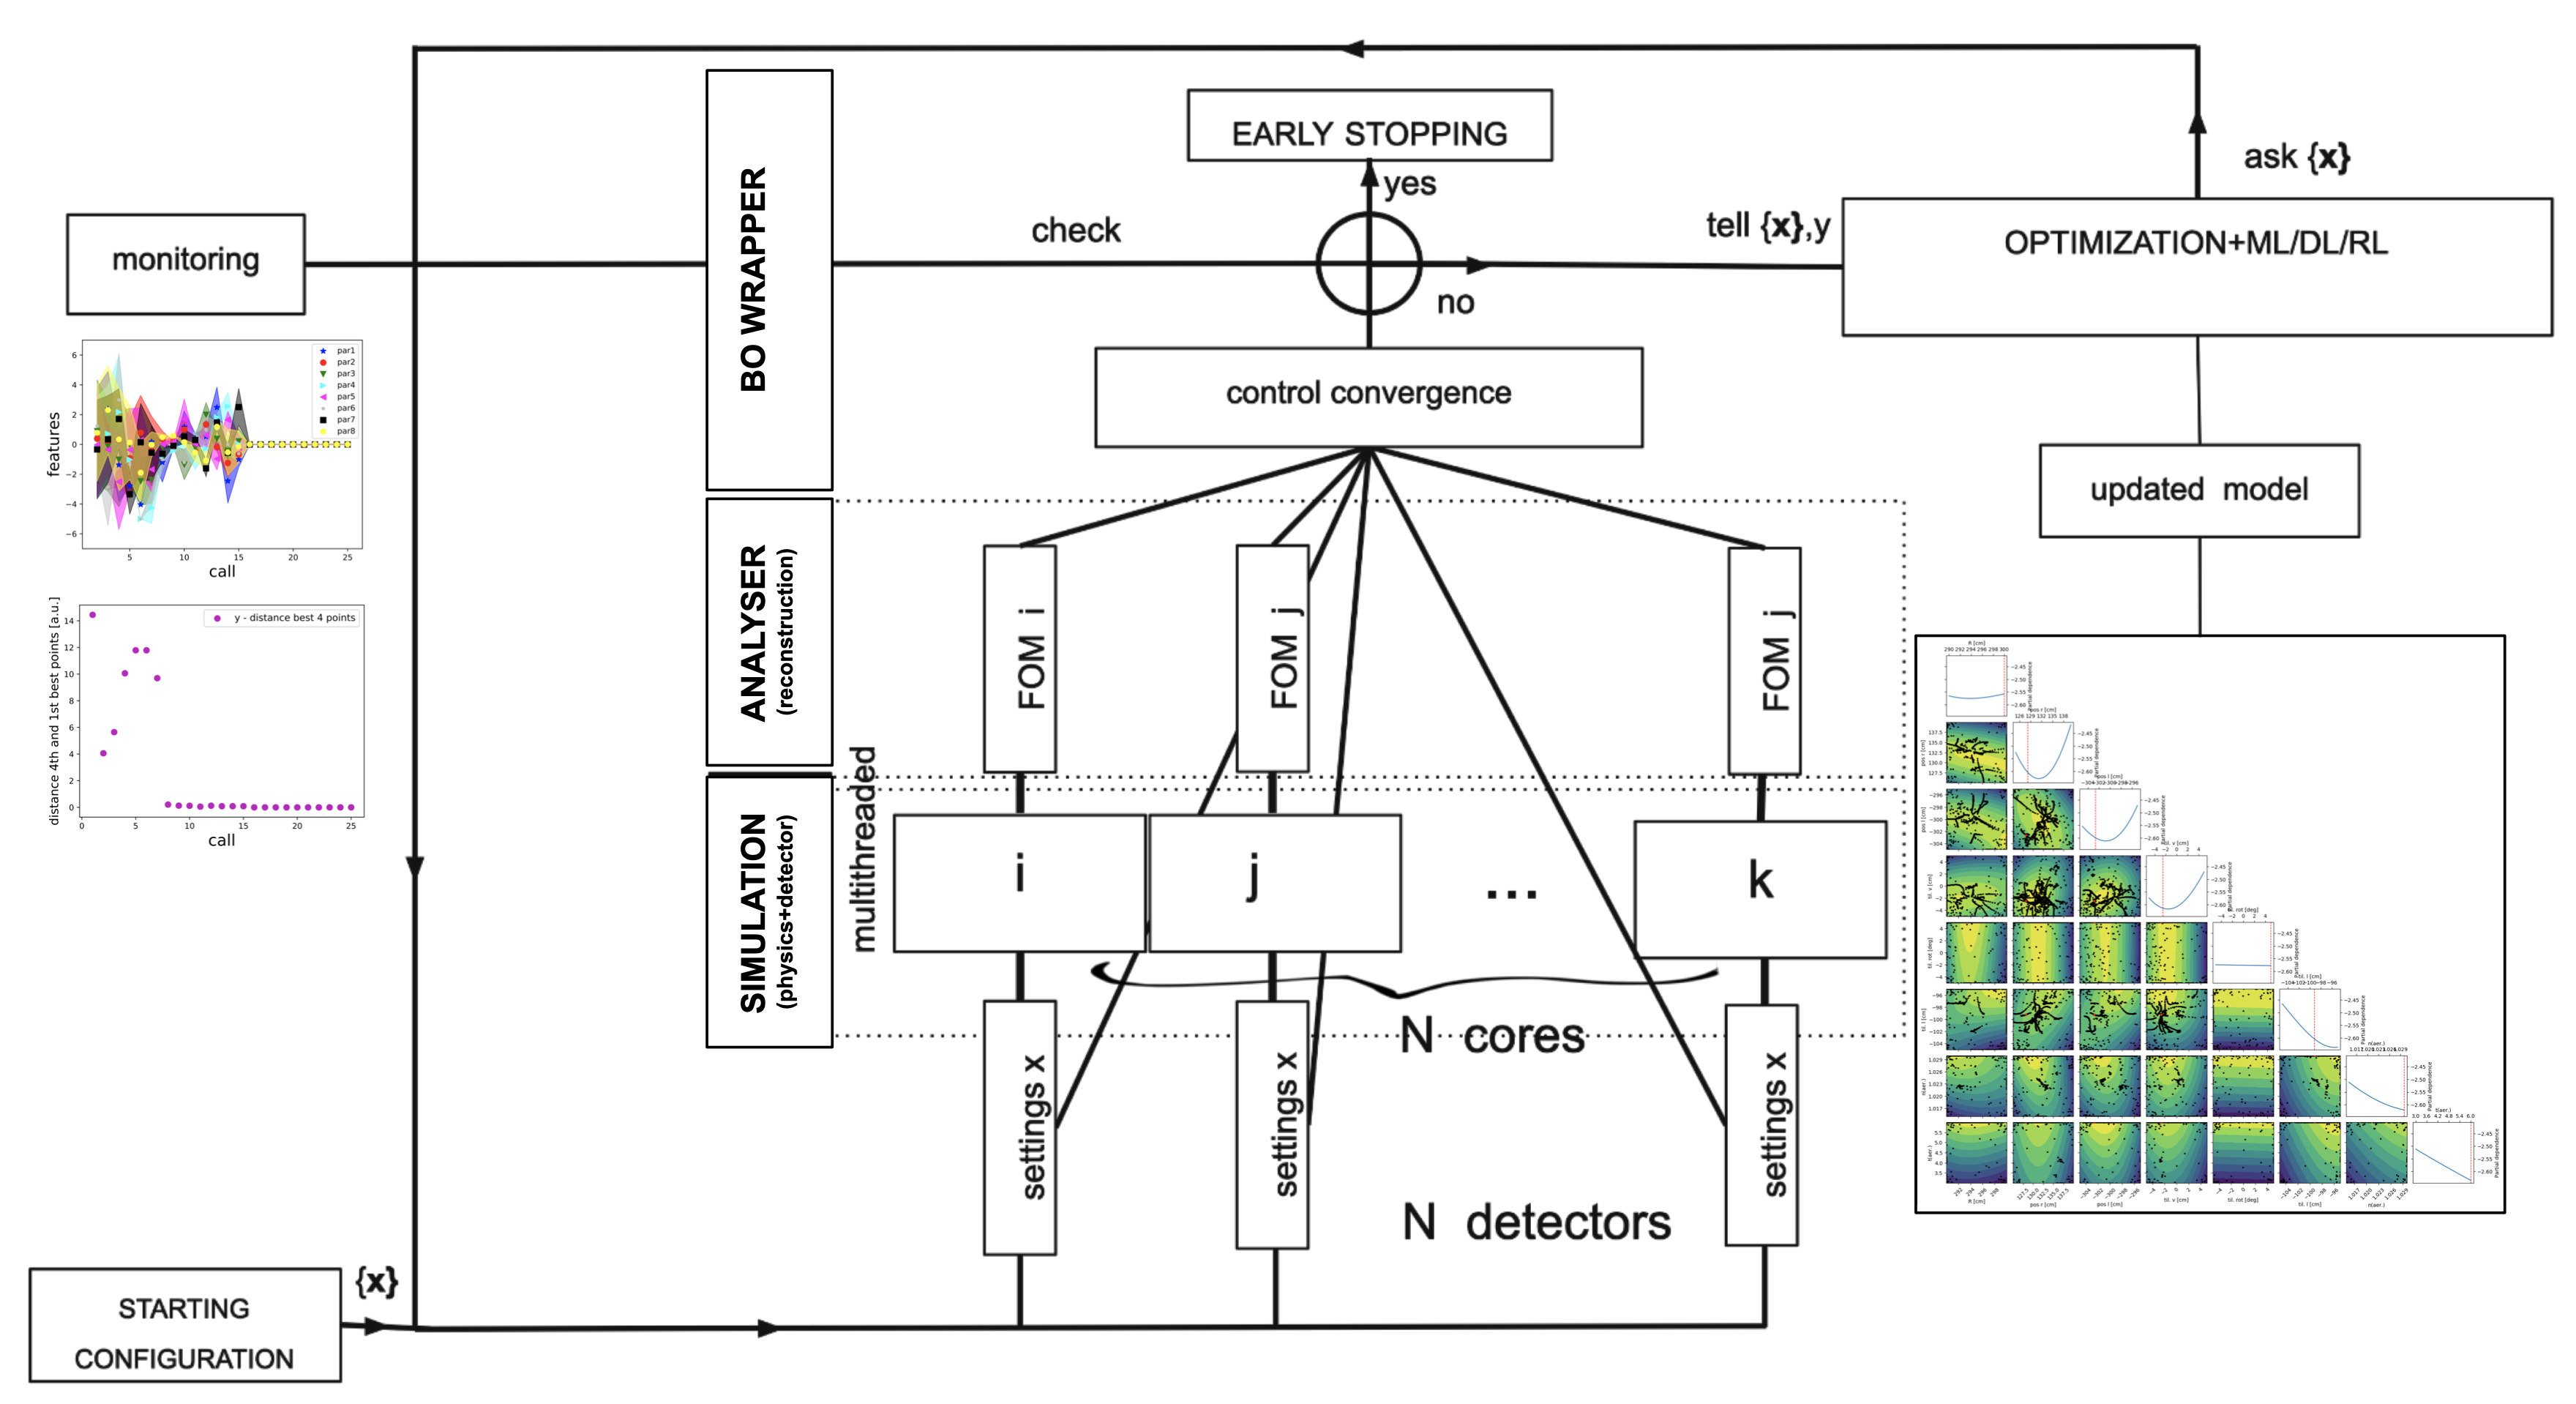
\includegraphics[scale = 0.21]{figs/dRICH_BO_scheme.png}
    \caption{
    Bayesian optimization framework for the optimization of the dual-RICH. N detector design points are created in parallel and passed to the BO which uses Gaussian processes, which collects the points, updates the surrogate model (a 2D visualization is shown in the bottom right corner considering all pairs of design parameters). A cheap acquisition function suggests a new set of design points to query at the next iteration. Convergence criteria are implemented on both the design space and on the objective (in this case, the $\pi$/K separation power of the dual-RICH) and early stopping is activated when convergence is observed in both spaces. Figure taken from \cite{fanelli_jluo2021}. More details can be found in \cite{cisbani2020ai}.   
    }
    \label{fig:dRICH_BO_scheme}
\end{figure}

An unprecedented study in detector design using AI has been accomplished during the detector proposal and a framework for multi-objective optimization of the ECCE design has been developed. 
Our approach deals with a complex optimization in a multidimensional design space driven by multiple objectives that encode the detector performance, while satisfying several mechanical constraints. 
This framework has been developed for the optimization of the Inner Tracker of ECCE but can be utilized in principle for any other sub-detector or system of sub-detectors, provided a viable parametrization of the detector simulation. 

The simulation and reconstruction relies on Fun4All \cite{fun4allGithub}, described later in Sec.~\ref{subsec:reconstruction}. 
Different parametrizations of the inner tracker design have been explored and most of our studies have been done with at least 11 parameters in the design space characterizing the location of the tracking layers in the central region and of the disks in the two endcaps (e-going and h-going directions), along with their dimensions and geometry. 
Eventually the parametrization has been extended to include also the support structure in the design optimization problem.   
Notice that potential overlaps among modules are checked before and during the optimization. 
The different designs have been optimized with particle gun samples of pions and then studied and validated with independent data samples and physics analyses.  

At least three objective functions have been optimized simultaneously. In particular for a 3-objective problem we utilized the momentum resolution, the polar angular resolution along with the Kalman filter (KF) efficiency of $\pi$ tracks. 
This multi-objective optimization (MOO) problem has been tackled with evolutionary algorithms. 
In this context, we used a recently developed framework for MOO called pymoo \cite{blank2020pymoo} which supports evolutionary multi-objective optimization algorithms such as Non-Dominated Sorting Genetic Algorithm (or NSGA-II, \cite{deb2002fast}). 
The NSGA workflow is described in Fig.~\ref{fig:NSGA_workflow}.
The main features of NSGA-II are (i) the usage of an elitist principle, (ii) an explicit diversity preserving mechanism, and (iii) ability of determining non-dominated solutions. 
%
The latter feature is of great importance for problems where objectives are of conflict to each other, that is: an improved performance in an objective results in worse performance in another objective.

\begin{figure}[!]
    \centering
    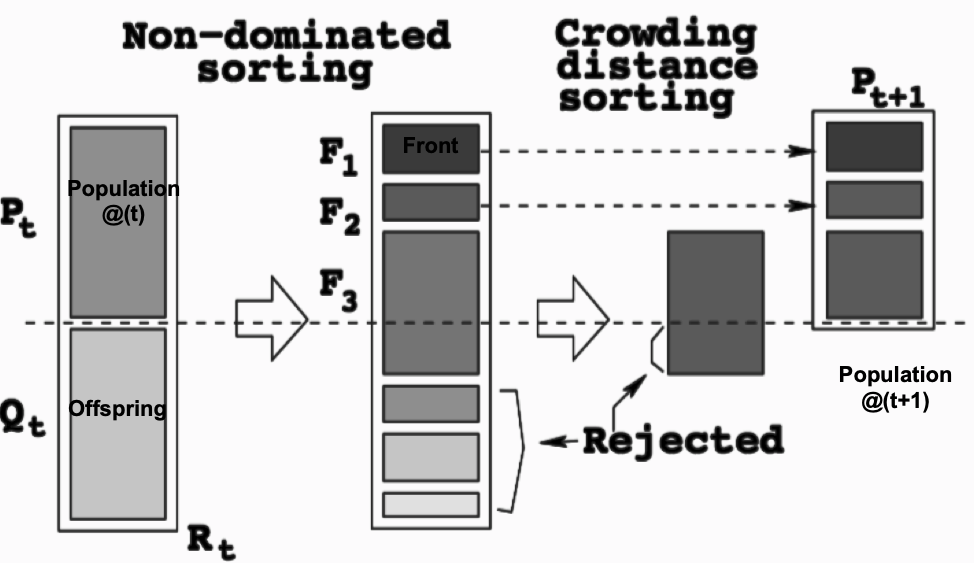
\includegraphics[scale = 0.35]{figs/NSGA_workflow2.png}
    \caption{The NSGA Workflow. At time $t$, an offspring is created through a genetic algorithm~\cite{whitley1994genetic} from an $N-$sized population of design points. 
    The two populations are combined into a population $R_{t}$, which is classified into different non-dominated classes $F_{i}$, starting from the first front $F_{1}$. 
    To restore the initial size of the population, the augmented space of solutions is trimmed. A metric called crowding distance is used to reject solutions and eventually provide an updated population of size $N$ at time $t+1$. 
    Image taken from \cite{deb2002fast}.
    }
    \label{fig:NSGA_workflow}
\end{figure}

Remarkably these approaches can accommodate mechanical and geometrical constraints during the optimization process. In our studies we included at least 5 constraints (\textit{e.g.}, the outermost location of a disk or a layer in the Inner Tracker, or the difference between the outer and inner radius of a disk) during the exploration of the design parameter space.  

A two-level parallelization has been implemented in the MOO framework: the first level creates the parallel simulations of design points, the second level parallelizes each design point. 
The evaluation itself can be distributed to several workers or a whole cluster with libraries like Dask \cite{dask}.

Computing time studies have been carried out to evaluate the simulation time of each single design point as a function of the number of tracks generated. 
Similarly we made studies of the computing time taken by the AI-based algorithm in generating a new population of design points. 
Results of these studies are summarized reported in Fig.~\ref{fig:computing-times}.  


\begin{figure}[!]
    \centering
    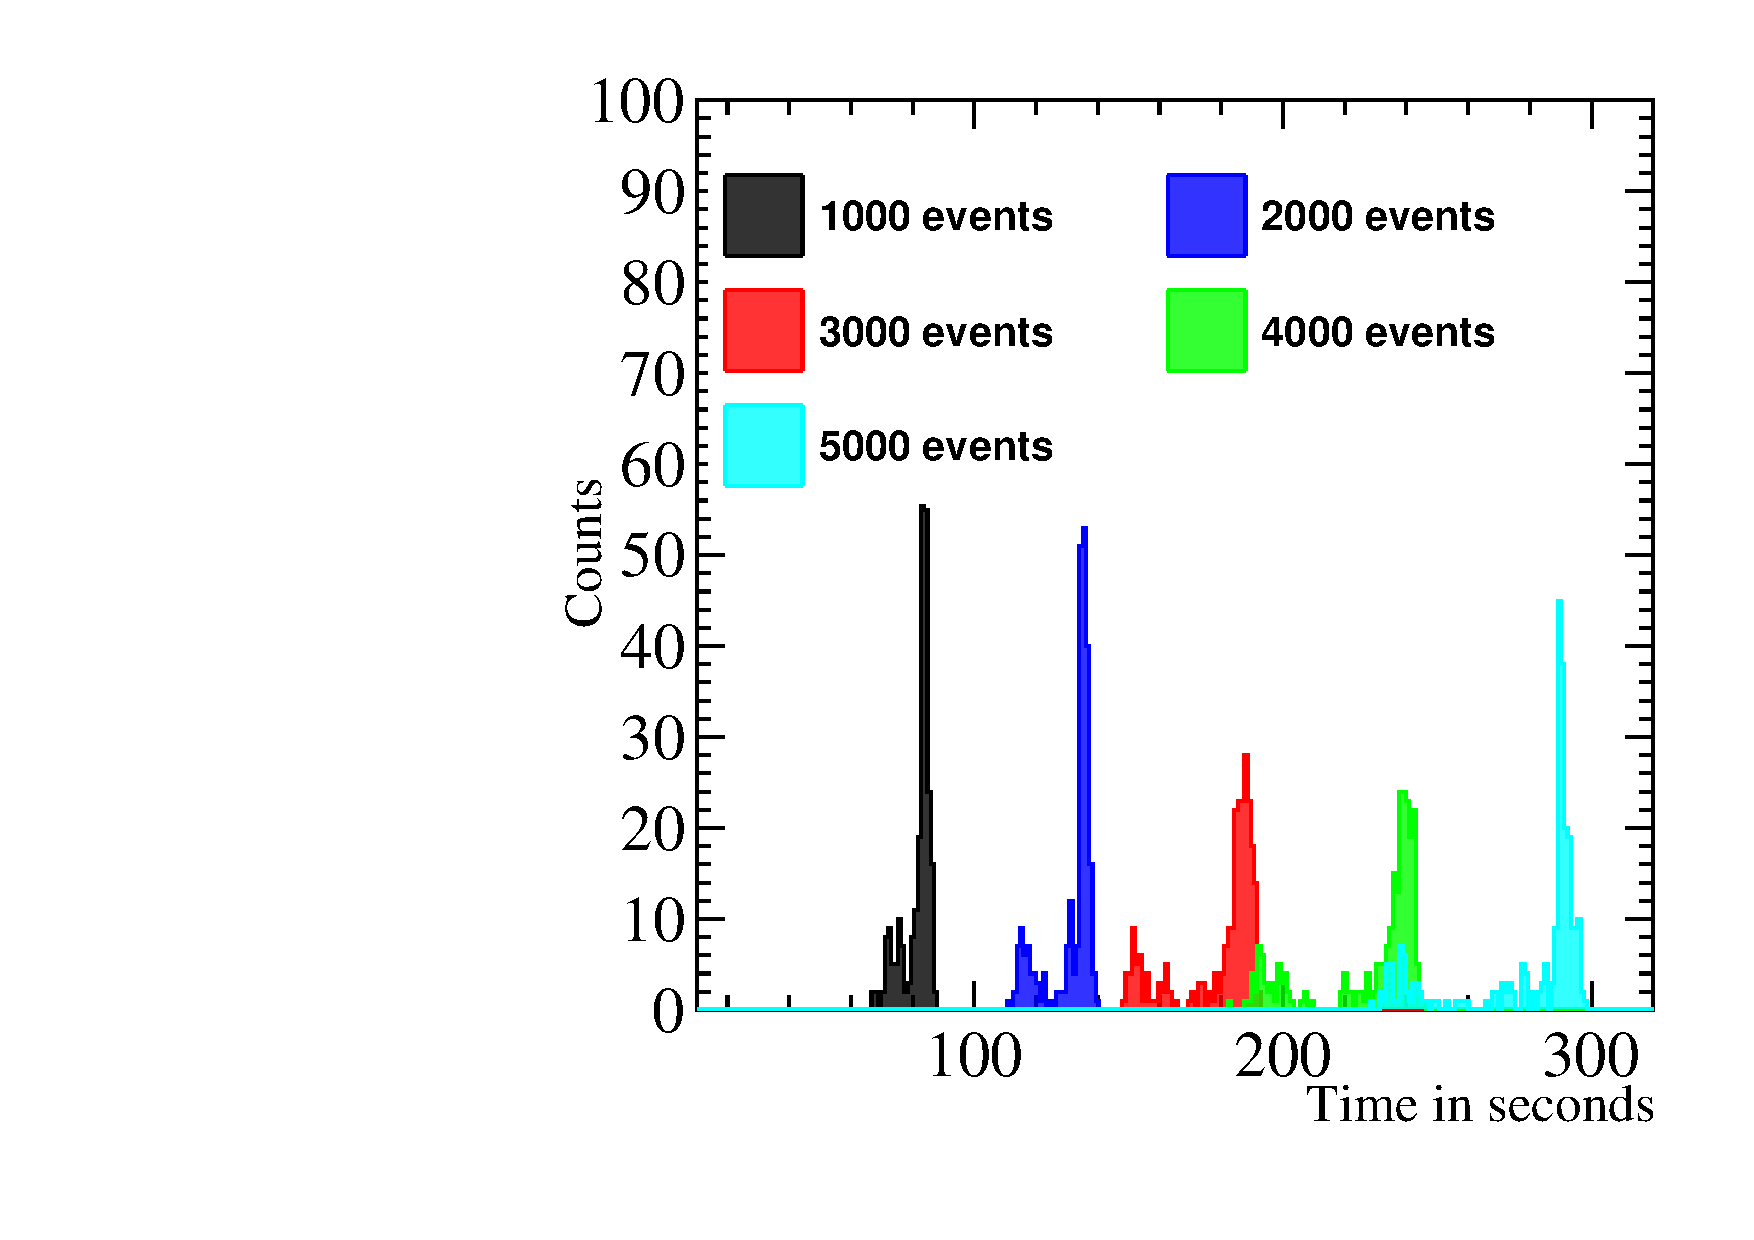
\includegraphics[scale = 0.33]{figs/TimeHistROOT.pdf}
    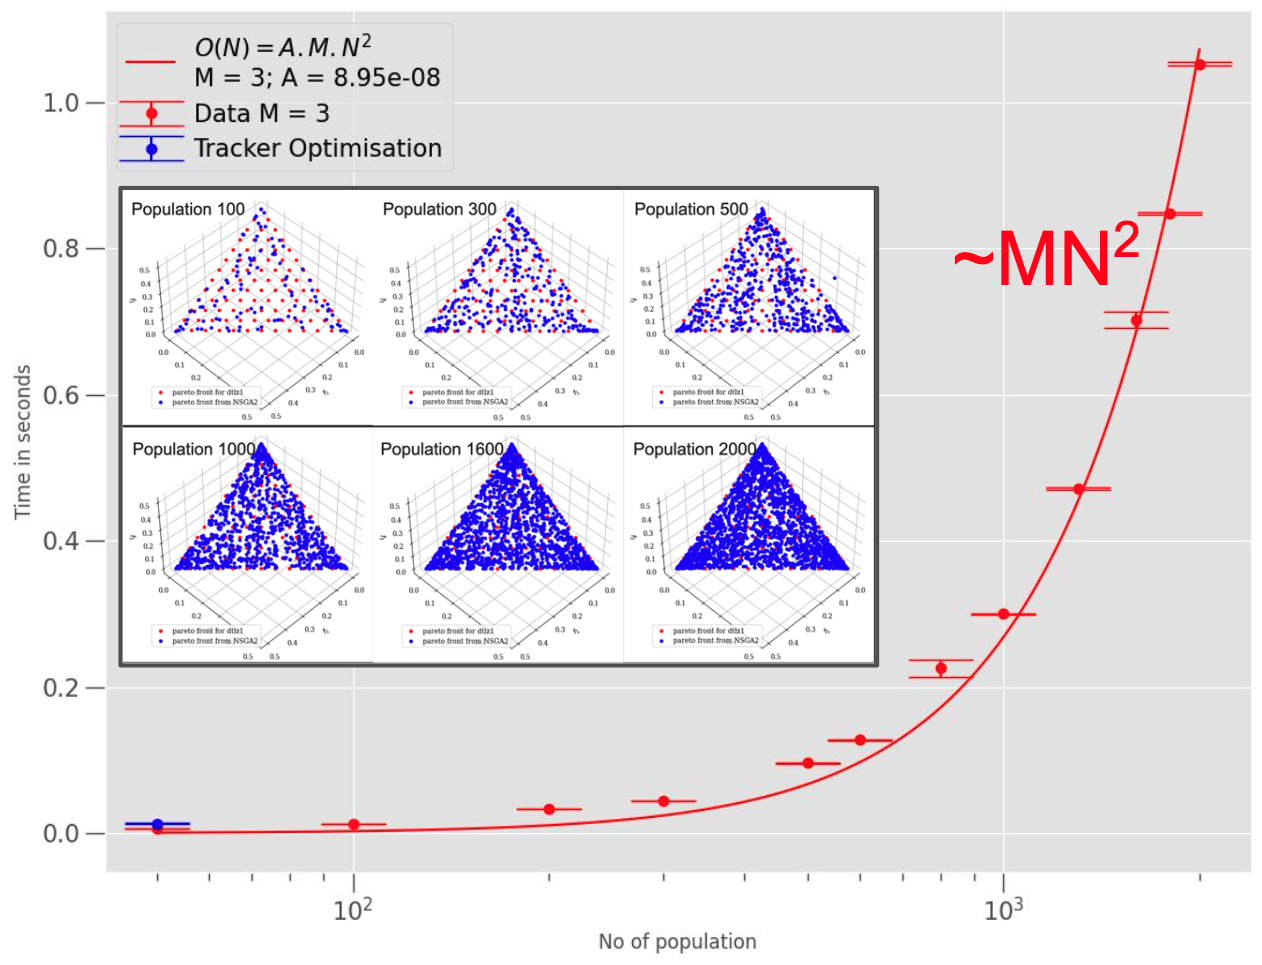
\includegraphics[scale = 0.18]{figs/AI_time_study.png}
    \caption{Computing time studies. (left) The simulation time of a single design point as a function of the number of tracks; (right) the computing time taken by the genetic algorithm and the sorting in NSGA-II. Performance have been benchmark with test problems like DTLZ1 \cite{ishibuchi2016performance} and the scaling $\sim MN^{2}$ has been verified with convergence to the Pareto front. For the complexity of the problem described in Table \ref{tab:complexity}, the simulation time dominates the AI times. A two level parallelization has been introduced in the framework to reduce this bottleneck.  
    The AI contribution typically becomes dominant when very a large population size is needed for an accurate approximation of the Pareto front. 
}
    \label{fig:computing-times}
\end{figure}

AI has played a crucial role in helping to choose a combination of technologies for the inner tracker, as shown in Fig. \ref{fig:improved_with_AI} (top). 
This is a dynamical/iterative process that evolves in time and requires the interplay between the ECCE teams working on Physics, Detector and Computing.
Results are validated by looking at figures of merit that do not enter as objective functions in the optimization process. The decision making is left post hoc and discussed among the Computing, Detector and Physics Teams, see Fig. \ref{fig:improved_with_AI} (bottom).


%The set up framework can be utilized for the optimization of other detectors too.

\begin{figure}[!]
    \centering
    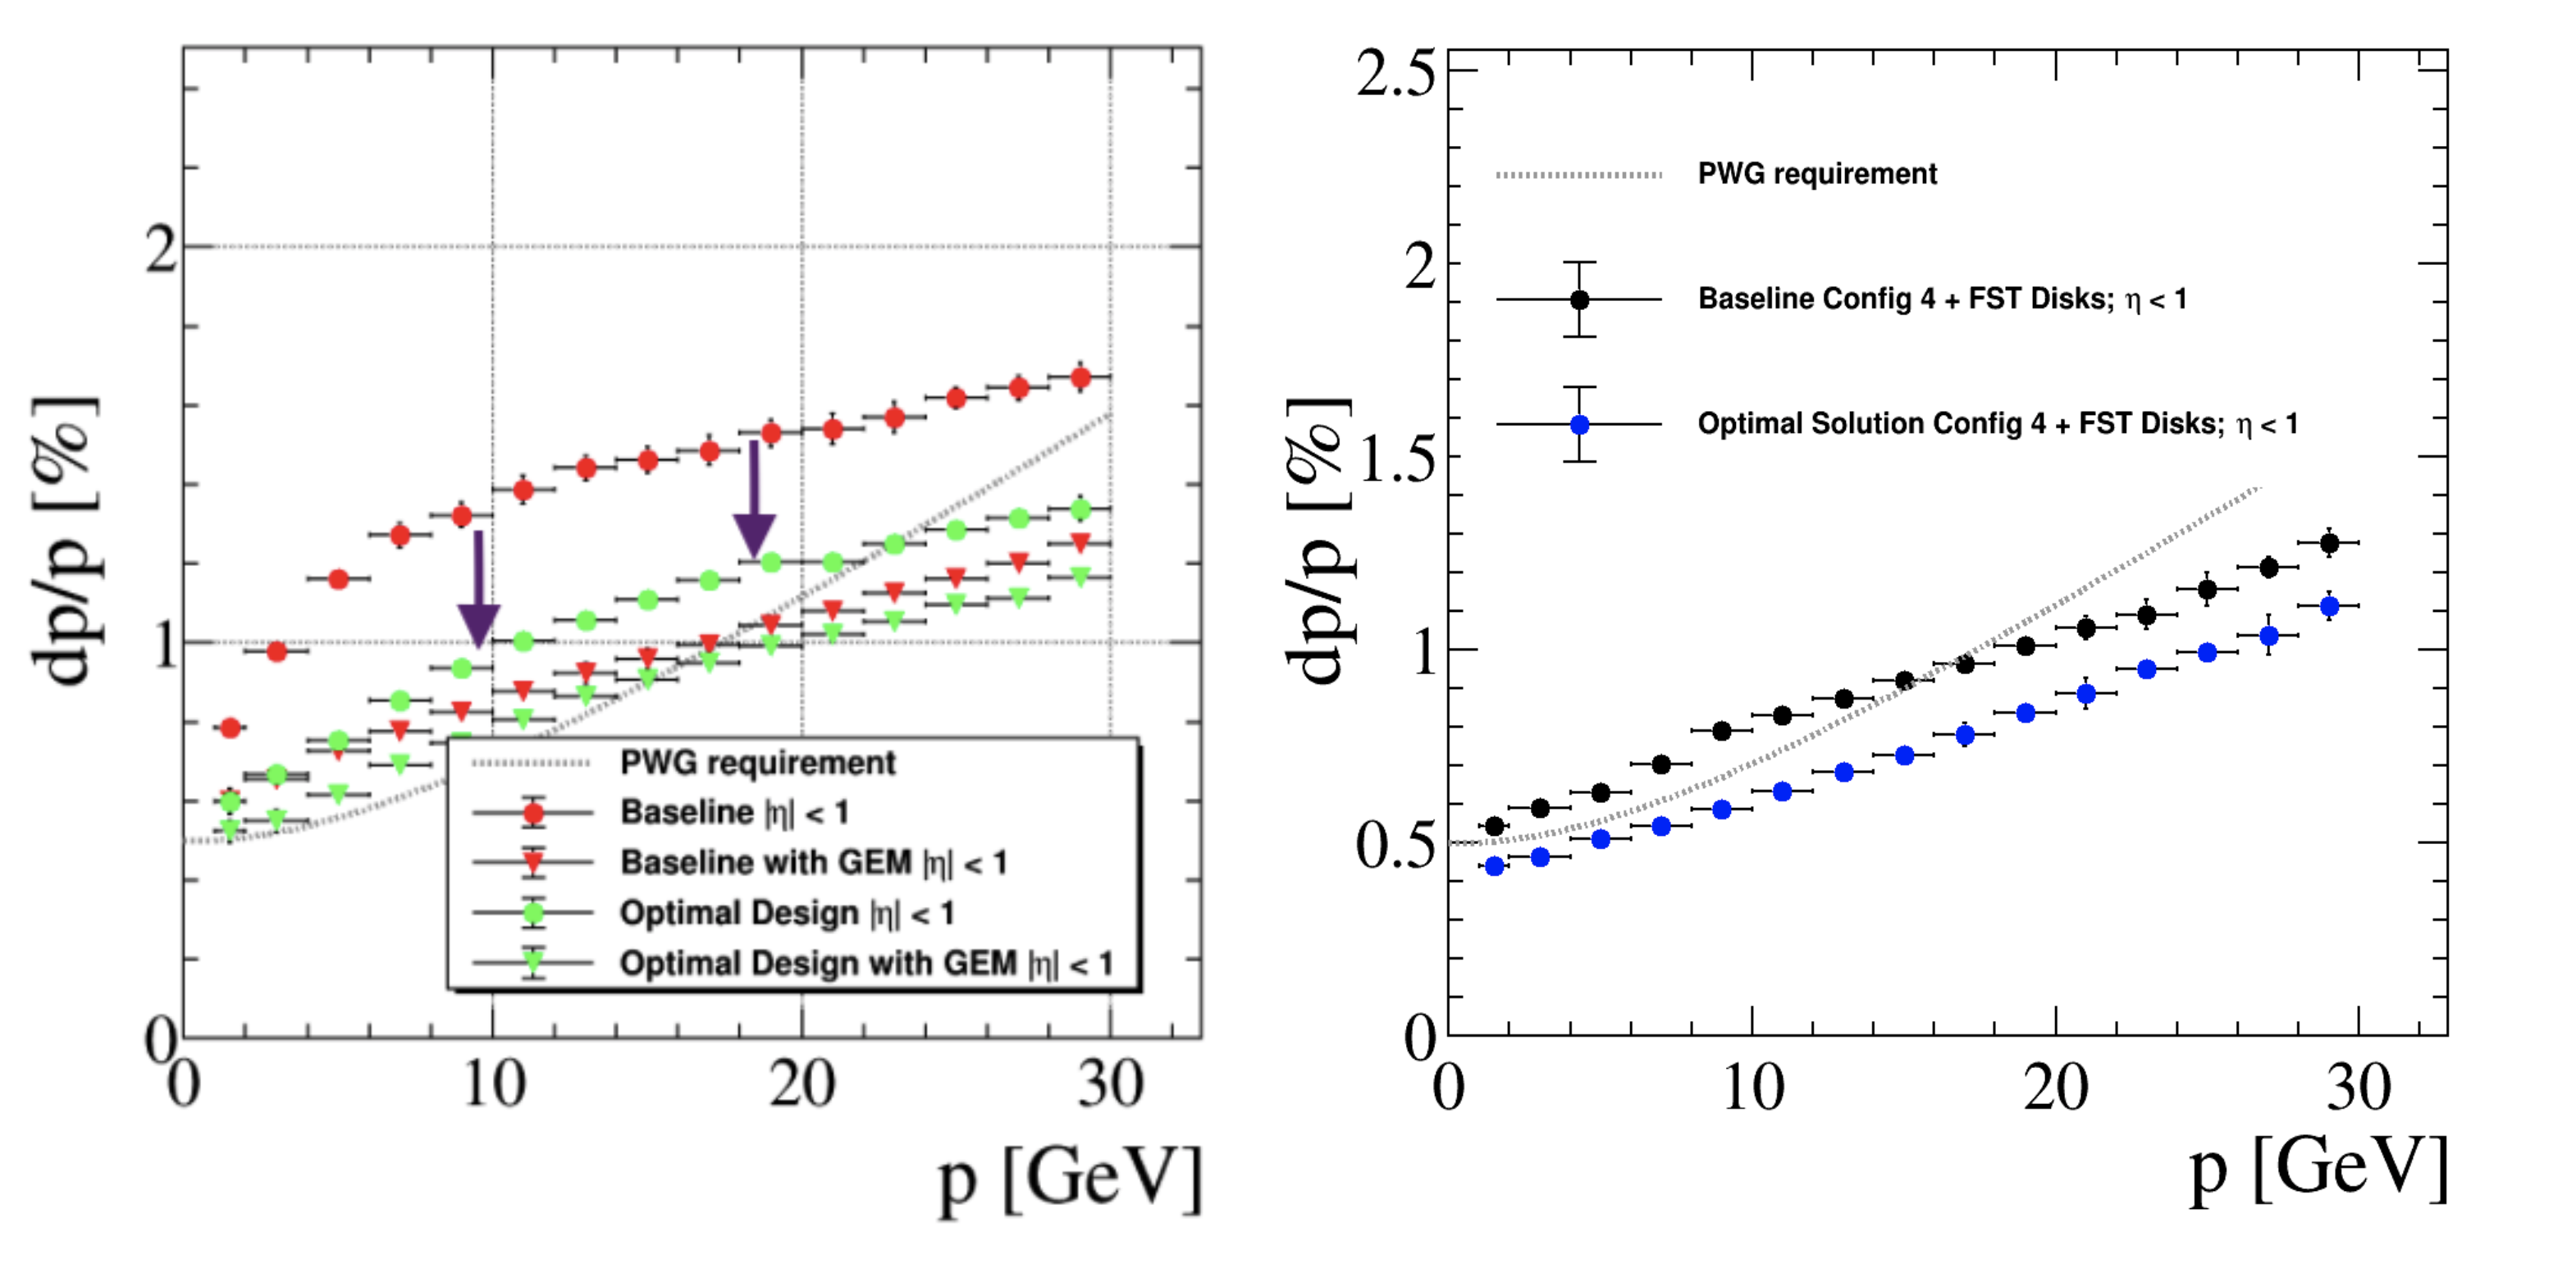
\includegraphics[scale = 0.26]{figs/improve_with_AI.png}
    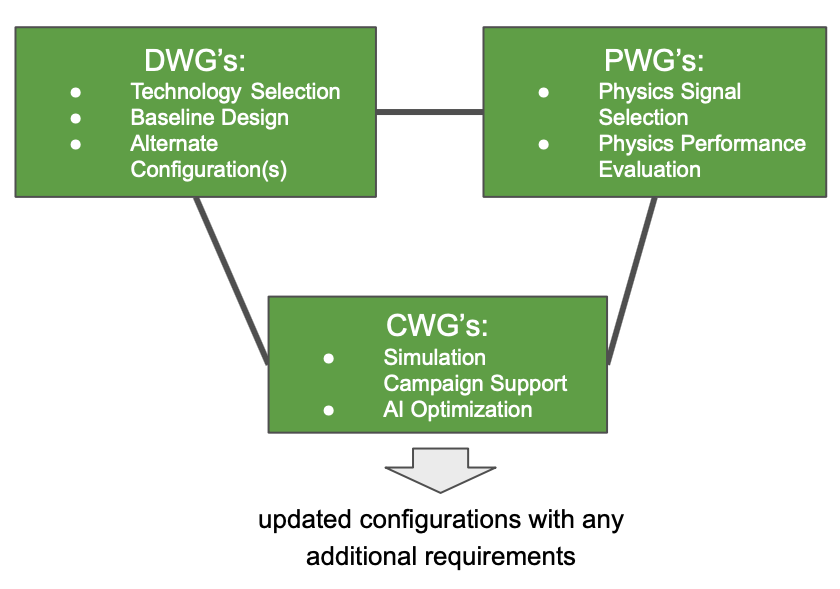
\includegraphics[scale = 0.36]{figs/interplay.png}
    \caption{
    Example of improvement in performance of the Inner Tracker barrel design during the detector proposal ascribable to Artificial Intelligence. AI took the red points (initial design) to green. The detector concept further evolved since then and AI improved it from black to blue by rearranging the geometry and dimensions of the components. It is clear that the fundamental interplay between the ECCE Teams working on Physics(PWG), Detector(DWG) and Computing(CWG) is propelled by AI in the design process. 
}
    \label{fig:improved_with_AI}
\end{figure}

The reader should be reminded that a Pareto front is potentially made by a set of trade-off solutions. Fig.~\ref{fig:convergence} shows the convergence plot obtained utilizing the hypervolume as metric, and a petal diagram with the three objectives corresponding to one solution in the Pareto front. 

\begin{figure}[!]
    \centering
    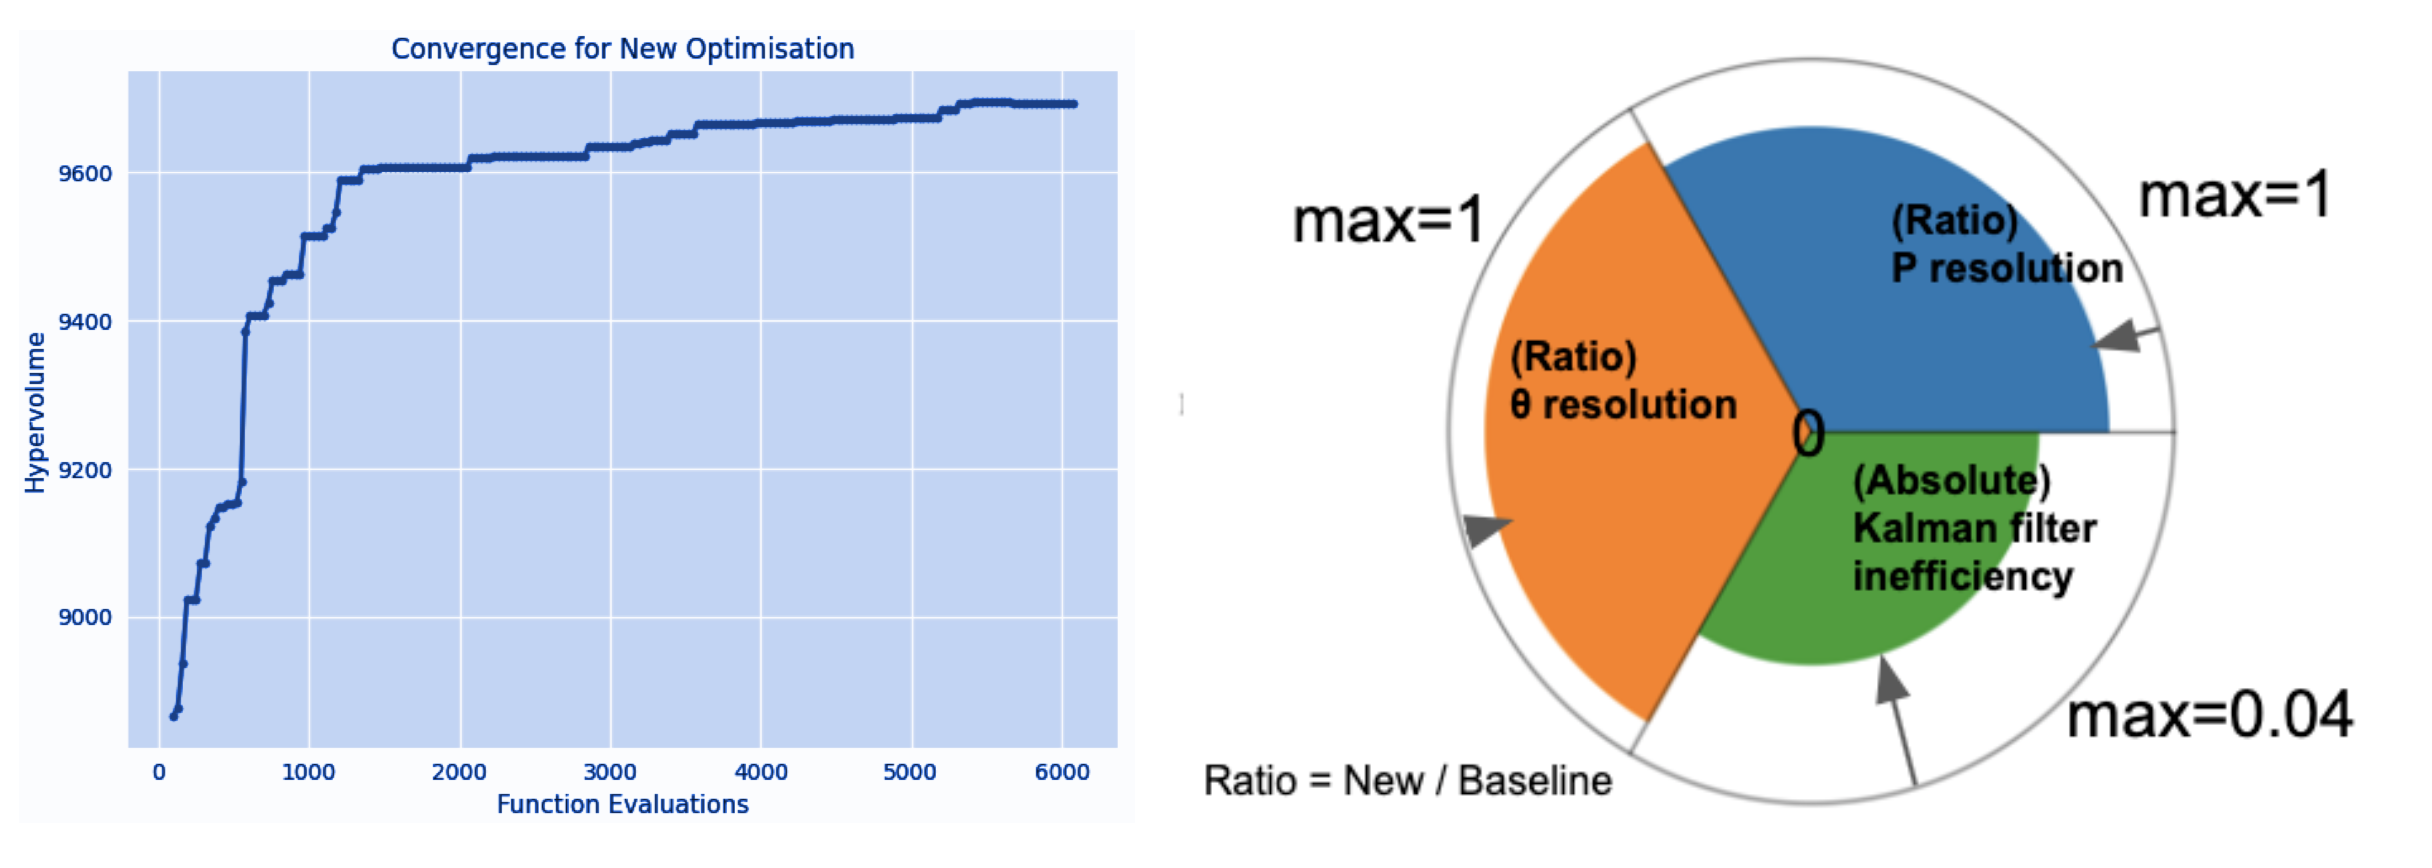
\includegraphics[scale = 0.35]{figs/convergence.png}
    \caption{(left) The hypervolume can be used as a metric for convergence. Checkpoints are created during the optimization and snapshots of the evolving designs can be taken. (right) A petal diagram with the three objectives corresponding to one solution in the Pareto front. The momentum and angular resolutions are expressed as ratios with respect to a baseline design to improve; the KF inefficiency is taken as an absolute value. An optimal design minimizes all of the above defined objectives. 
}
    \label{fig:convergence}
\end{figure}

A complete list of the hyperparameters of our optimization framework can be found in Table \ref{tab:complexity}.
With 11 variables and 3 objectives it has been estimated that approximately $\sim$10k core-hours on CPU is needed to converge. 
%
This number is expected to grow with the complexity of the problem,  which is characterized by the number of design parameters and objectives. 
%which in turn may require larger populations and more iterations to approach convergence and approximate the Pareto front. 
%
%%This approach can be further utilized 
%%We describe our strategy and show preliminary results for the Si tracking system. 
%
Larger populations of design points can be simulated to improve accuracy of the Pareto front in multidimensional spaces with AI-based accelerated optimizations. 
An interesting trend is scaling the MOO workflows on HPC systems \cite{liu2020parallelization}. 

Remarkably the developed framework can be utilized for other sub-detectors, or systems of sub-detectors.


\begin{table}[!]
    \centering
    \begin{tabular}{|M{3.cm} | M{3.5cm}| M{2.0cm}|}
        \hline
        \textbf{description} & \textbf{symbol} & \textbf{value} \\ 
        \hline
        \hline
        \small{population size} & N & 100 \\
        \small{\# objectives}   & M & 3(4)\\ 
        \small{offspring} & O & 30(50)\\
        \small{design size} & D & 11(16) \\
        \small{\# calls (tot. budget)} & $-$ & 200\\
        \small{\# cores} & $-$ & \small{same as offspring} \\
        \small{\# charged $\pi$ tracks} & N$_{\textup{trk}}$ & 80k\\
        \small{\# bins in $\eta$} & N$_{\eta}$ & 3 \\
        \small{\# bins in P} & N$_{\textup{P}}$ & 15 \\
        \hline
    \end{tabular}
    \caption{Summary of the hyperparameters during the optimization. Symbols used throughout the document to describe these quantities are also reported to facilitate the reader. Values not in parentheses correspond to the optimization of a starting reference design. Values in parentheses are the largest ones utilized in other optimization pipelines. Checkpoints are created allowing to take a snapshot of the optimization while ongoing. A survey of the detector performance is created after each call. At each call an offspring of 30 to 50 new design points is created through a genetic algorithm. A two-level parallelization is implemented as explained in the text. The framework ran on the JLab computing farm which currently host nodes with a maximum number of 128 cores.
    }
    \label{tab:complexity}
\end{table}




\clearpage